%% IEEE BigData 2026 -- 3rd High School Symposium
%% Compile on Overleaf with the IEEEtran document class (conference mode).
\documentclass[conference]{IEEEtran}
\IEEEoverridecommandlockouts
\usepackage{cite}
\usepackage{amsmath,amssymb,amsfonts}
\usepackage{algorithmic}
\usepackage{graphicx}
\usepackage{textcomp}
\usepackage{booktabs}
\usepackage{xcolor}
\def\BibTeX{{\rm B\kern-.05em{\sc i\kern-.025em b}\kern-.08em T\kern-.1667em\lower.7ex\hbox{E}\kern-.125emX}}

\begin{document}

\title{Stability Selection Without Repeated Refitting:\\
Refit-Free Selection Stability and Empirical FDR Control\\
from a Single Model Fit}

\author{\IEEEauthorblockN{Hrudhai Lothumalla}
\IEEEauthorblockA{\textit{Heritage High School}, Frisco, TX, USA \\
\textit{AIEA Lab, University of California, Santa Cruz}\\
Santa Cruz, CA, USA}
\and
\IEEEauthorblockN{Eshaan Nidee}
\IEEEauthorblockA{\textit{Liberty High School}, Frisco, TX, USA \\
\textit{AIEA Lab, University of California, Santa Cruz}\\
Santa Cruz, CA, USA}
\and
\IEEEauthorblockN{Leilani Gilpin}
\IEEEauthorblockA{\textit{AIEA Lab} \\
\textit{University of California, Santa Cruz}\\
Santa Cruz, CA, USA \\
lgilpin@ucsc.edu}}

\maketitle

\begin{center}\vspace{-0.9em}\small\textit{Hrudhai Lothumalla and Eshaan Nidee
contributed equally to this work and are co-first authors.}\end{center}
\vspace{0.4em}

\begin{abstract}
Reproducible, error-controlled feature selection is a core data-mining task, but
the dominant tool, stability selection, estimates how often each feature is
chosen by refitting the model on hundreds of subsamples, a cost that is
prohibitive at scale. We ask whether stability-selection-grade behavior can be
obtained from a single model fit, reusing the bootstrap resampling that a random
forest already performs internally rather than adding an outer refitting loop.
We contribute SF-Select, which fits one random forest on the data augmented with
shadow (randomly permuted) features and applies a knockoff-plus style threshold
to the resulting importances. We are explicit that permutation shadows satisfy
the knockoff exchangeability conditions only approximately, so we do not claim a
proven finite-sample guarantee; we instead treat false-discovery-rate control as
an empirical property and map its operating regime over a thirty-seed grid. The
map is itself the finding: with near-independent features the realized false
discovery rate is controlled and SF-Select exceeds complementary-pairs stability
selection (CPSS) on power at roughly fourteen times less compute, but under
correlated features the shadow calibration fails and the false discovery rate
inflates sharply; under moderate correlation CPSS still controls the error,
while under the near-duplicate correlations of a real dataset even CPSS does not.
Independently, and robustly to correlation, we establish a law useful on its
own: a forest's between-tree dispersion of its per-feature importances is a
strong refit-free proxy for the true cross-resample standard deviation of the
importance (Pearson correlation 0.89 on synthetic data, and 0.95 and 0.72 on two
real datasets), consistently beating the infinitesimal jackknife; we use it to
annotate each selection with a stability score. We also report two honest
negative results that sharpen the method: the jackknife loses to simple
dispersion, and normalizing importances by dispersion nearly halves power.
Finally, clustering correlated features and selecting at the group level restores
false-discovery control in the correlated regime, trading feature-level for
cluster-level resolution. The contribution is domain-independent.
\end{abstract}

\begin{IEEEkeywords}
feature selection, false discovery rate, stability selection, random forests,
reproducibility
\end{IEEEkeywords}

\section{Introduction}
High-dimensional data mining routinely ends in a question of the form
\emph{which features matter?} The answer must be (a) \emph{reproducible}, meaning
the selected set should not swing wildly under resampling, and (b)
\emph{error-controlled}, meaning the fraction of falsely selected features should
be bounded. \emph{Stability selection}~\cite{meinshausen2010} and its
complementary-pairs refinement (CPSS)~\cite{shah2013} are the standard answer:
refit a base selector on many subsamples, keep features chosen with high
frequency, and bound the expected number of false selections. This is effective
but expensive: reproducibility is bought with $O(B)$ model refits
($B{=}100$--$1000$). At BigData scale, with many samples, many features, or an
expensive base learner, the refit tax is the bottleneck, and a wave of
2025--26 work continues to pay it~\cite{robustmodelmaker}.

The cost is not incidental. Reproducibility is the reason stability selection
exists: a single fit of a high-variance base learner can return a very different
top-$k$ set on a resampled version of the same data, and the biomarker-discovery
literature documents exactly this volatility across cohorts. Stability selection
tames it by keeping only features chosen consistently across many perturbed fits,
which is principled but converts one model fit into hundreds. On a large forest or
boosted ensemble, or on a stream that cannot be revisited, that multi-fit loop is
precisely what does not scale. This tension between reproducibility and cost is
the practical problem we target.

We ask a simple question: \emph{is the multi-fit resampling actually necessary
to see how (un)stable a feature's importance is?} A random forest already
contains $B$ trees trained on bootstrap resamples of the data. We show that the
\emph{dispersion of a feature's importance across those trees} is, by itself, a
strong refit-free estimate of how much that importance would move across
independent datasets. This lets us recover the reproducibility signal of
stability selection from a \emph{single} fit.

\noindent\textbf{Contributions.}
\begin{itemize}
\item \textbf{\textsc{SF-Select} (Sec.~\ref{sec:method}).} A single-fit
selection procedure with \emph{empirically verified} FDR control:
shadow-feature augmentation plus a knockoff\textsuperscript{+}-style threshold on
one forest's importances. It is an $O(1)$-refit drop-in for stability selection
and handles overlapping groups. We are explicit that the theoretical knockoff
guarantee is \emph{not} established for permutation shadows.
\item \textbf{The between-tree dispersion law (Sec.~\ref{sec:validity}).} A
forest's between-tree dispersion $s_j$ tracks the true cross-resample standard
deviation of its importance ($r{=}0.89$) and beats the infinitesimal jackknife
($r{=}0.55$); we use it as a free, validated per-feature stability annotation.
\item \textbf{Evidence, an operating map, and a fix (Sec.~\ref{sec:exp}).} On
synthetic and real data, \textsc{SF-Select} controls FDR and exceeds CPSS power
at a $14\times$ speedup \emph{in low-correlation designs}; we map where it breaks
(correlated features), then show that \emph{clustering features and selecting at
the group level restores FDR control} there. We also report two negatives (the
jackknife loses to simple dispersion; normalizing by dispersion halves power).
Honest scope is part of the claim.
\end{itemize}

\section{Problem Formulation}\label{sec:formulation}
We observe $\mathcal{D}=\{(x_i,y_i)\}_{i=1}^n$, $x_i\in\mathbb{R}^p$, i.i.d.\
from unknown $P$, with an unknown \emph{relevant set}
$\mathcal{R}^\star$; the rest $\mathcal{N}^\star$ are null. A rule returns
$\hat{\mathcal{S}}$; we target the false discovery rate
$\mathrm{FDR}=\mathbb{E}[\,|\hat{\mathcal{S}}\cap\mathcal{N}^\star|/
\max(1,|\hat{\mathcal{S}}|)\,]\le q$ at high power
$\mathbb{E}[|\hat{\mathcal{S}}\cap\mathcal{R}^\star|/|\mathcal{R}^\star|]$ and
high \emph{selection stability} (large Jaccard overlap of the sets chosen on
independent draws from $P$). Groups (possibly overlapping) are an optional
generalization.

\section{Background}\label{sec:bg}
We use three standard ingredients, recalled here to fix notation.
\emph{Out-of-bag (OOB) permutation importance.} In a bootstrap forest each tree
$b$ is trained on a resample of $\mathcal{D}$ and leaves roughly a third of the
rows unused (its OOB set). Permuting column $j$ in the OOB rows and measuring the
resulting drop in that tree's OOB accuracy gives a per-tree importance
$\phi_j^{(b)}$ that is (approximately) zero-mean for a truly null feature,
because permutation destroys any association without changing marginal
statistics. Averaging over trees yields the forest importance $\phi_j$.
\emph{Shadow features.} A shadow of column $j$ is a random permutation of that
column; it preserves the marginal distribution but severs the link to the label,
so it is null by construction. Comparing a real feature against shadows is the
idea behind Boruta~\cite{boruta}, used there as a heuristic cutoff.
\emph{The knockoff\textsuperscript{+} threshold.} Given a statistic $W_j$ that is
large for signal and symmetric for null features, Barber and
Cand\`es~\cite{barber2015} select $\{j: W_j\ge t^\star\}$ with
$t^\star=\min\{t:(1+\#\{{\rm null}\ W\ge t\})/\max(1,\#\{{\rm real}\ W\ge t\})\le
q\}$, which controls FDR at $q$ \emph{provided} the null statistics are
exchangeable with their negatives. \textsc{SF-Select} combines these three: it
scores features by a forest importance, calibrates against shadows, and thresholds
with the knockoff\textsuperscript{+} rule, all from one fit. The open question,
which the exchangeability caveat makes empirical rather than settled, is how
close permutation shadows come to the conditions the guarantee requires.

\section{Related Work and the Gap}\label{sec:related}
\emph{Stability selection}~\cite{meinshausen2010} and CPSS~\cite{shah2013} bound
false selections via subsample selection \emph{frequencies}; every variant,
including recent pipelines~\cite{robustmodelmaker}, requires many refits.
Covert--Lee~\cite{covert2021} give the \emph{Monte-Carlo} variance of KernelSHAP
\emph{estimators} (noise in estimating one model's attribution, not its
variability across datasets). Wager et al.~\cite{wager2014} estimate the
sampling variance of random-forest \emph{predictions} refit-free from in-bag
counts; we repurpose that machinery for \emph{attributions} but find a simpler
dispersion statistic works better (Sec.~\ref{sec:validity}).
Barber--Cand\`es~\cite{barber2015} give finite-sample FDR via a
knockoff\textsuperscript{+} threshold and Model-X knockoffs~\cite{candes2018}
extend it, but both need a sampled knockoff distribution; Boruta~\cite{boruta}
uses shadow (permuted) features heuristically, without FDR guarantees.
\emph{Our question} is empirical: can the internal bootstrap structure of a
\emph{single} forest supply the reproducibility and error-control signal that
stability selection buys with $O(B)$ refits? We measure, not assume, the answer.

\section{The Between-Tree Dispersion Law}\label{sec:validity}
Let $f$ be a random forest of $B$ trees; tree $b$ is trained on a bootstrap
resample and yields a per-tree attribution $\phi_j^{(b)}$ for feature $j$
(we use out-of-bag permutation importance). The forest attribution and its
between-tree dispersion are
\begin{equation}
\phi_j=\frac1B\sum_{b=1}^B \phi_j^{(b)},\qquad
s_j^2=\frac{1}{B-1}\sum_{b=1}^B\big(\phi_j^{(b)}-\phi_j\big)^2 .
\end{equation}
The quantity we \emph{want} is the cross-resample standard deviation
$\sigma_j=\mathrm{SD}_{\mathcal{D}\sim P}(\phi_j)$, which normally requires
refitting on many datasets. \emph{Claim:} $s_j$ is a strong refit-free proxy
for $\sigma_j$. Intuitively, the trees are trained on bootstrap resamples of
$\mathcal{D}$, so their spread reflects sensitivity to the data; a feature whose
importance is fragile across trees is fragile across datasets. We validate this
directly (Sec.~\ref{sec:exp}, Fig.~\ref{fig:validity}): across features,
$\mathrm{corr}(s_j,\sigma_j)=0.89$, whereas the bias-corrected IJ estimate
attains only $0.55$ because its $-(n/B)$ Monte-Carlo correction is high-variance
at practical $B$; the law is confirmed on real data ($r{=}0.95$ and $0.72$, E7).
We therefore build on $s_j$, not the IJ.

\emph{Why does the spread transfer?} Two sources contribute to how a forest
importance moves. The first is Monte-Carlo noise from the finite OOB set and the
finite number of trees, which vanishes as $B$ grows. The second is the
sensitivity of the learned splits to \emph{which} data points are present; a
feature that is used near the root of many trees regardless of the resample has
low between-tree spread, while a feature that only occasionally wins a split has
high spread. Because each tree sees a bootstrap resample, the second component is
already a within-fit Monte-Carlo estimate of the same data-perturbation
sensitivity that stability selection measures with an outer resampling loop. The
infinitesimal jackknife tries to isolate this component analytically from the
in-bag counts, but at practical $B$ its bias correction subtracts two large,
noisy quantities and the estimate degrades; the raw dispersion keeps both
components and, empirically, ranks features far more faithfully. This is why the
simpler statistic wins, and why we treat $s_j$ as a reproducibility annotation
rather than a normalizer (normalizing by it demotes strong, high-spread signals;
see E3).

\section{SF-Select}\label{sec:method}
\emph{Selection statistic.} The selection statistic is the forest importance
$\phi_j$ itself. (We tested the between-tree $t$-ratio $\phi_j/(s_j+\varepsilon)$
as an alternative; Sec.~\ref{sec:exp} shows it \emph{hurts}, so \textsc{SF-Select}
selects on $\phi_j$ and reserves $s_j$ for annotation.)
\emph{Null calibration.} We augment the design with $p$ \emph{shadow}
features, each a random permutation of a randomly chosen real column; shadows are
guaranteed null and provide an empirical null without label-permutation refits.
We fit the forest \emph{once} on the augmented design and compute $\phi_j$ for
real and shadow features. \emph{FDR control.} Following the
knockoff\textsuperscript{+} rule~\cite{barber2015}, for threshold $t$ let
\begin{equation}
\widehat{\mathrm{FDP}}(t)=\frac{1+\#\{j\in\mathrm{shadow}:\phi_j\ge t\}}
{\max\!\big(1,\#\{j\in\mathrm{real}:\phi_j\ge t\}\big)},
\end{equation}
choose $t^\star=\min\{t:\widehat{\mathrm{FDP}}(t)\le q\}$, and select real
features with $\phi_j\ge t^\star$.

\emph{Theoretical status (stated plainly).} The knockoff\textsuperscript{+}
rule provably controls FDR \emph{when} null-real and shadow statistics are
exchangeable~\cite{barber2015}. Model-X knockoffs~\cite{candes2018} secure this
by \emph{sampling} a knockoff distribution; our shadows are cheap
\emph{permutations} (Boruta-style~\cite{boruta}) and satisfy exchangeability only
approximately, so \emph{we do not claim the theorem holds for our
construction.} We adopt the threshold as a heuristic and \emph{measure} the
realized FDR (Sec.~\ref{sec:exp}). \emph{Stability annotation.} Each selected feature is
reported with its between-tree dispersion $s_j$ (Sec.~\ref{sec:validity}), a
validated refit-free estimate of how much its importance would move on a fresh
cohort. \emph{Groups.} For a group $g$, $\phi_g^{(b)}$ is the per-tree
importance of jointly permuting all members of $g$; group shadows (permuted
group blocks) follow identically, giving group-level FDR that respects overlap.

\begin{algorithm}[t]
\caption{\textsc{SF-Select} (single fit)}
\begin{algorithmic}[1]
\STATE \textbf{Input:} data $(X,y)$, forest size $B$, level $q$
\STATE $\tilde X\leftarrow[\,X \mid \mathrm{Shadows}(X)\,]$ \hfill// permuted null columns
\STATE fit one random forest $f$ with $B$ bootstrap trees on $(\tilde X,y)$
\FORALL{tree $b$}
\STATE $\phi^{(b)}_\cdot\leftarrow$ OOB permutation importance (all columns)
\ENDFOR
\STATE $\phi_j\leftarrow\mathrm{mean}_b\,\phi^{(b)}_j$;\;
       $s_j\leftarrow\mathrm{SD}_b\,\phi^{(b)}_j$ \hfill// $s_j$ = stability annotation
\STATE $t^\star\leftarrow$ knockoff\textsuperscript{+} threshold on
       $\{\phi_j\}$ at level $q$
\STATE \textbf{return} $\{(j,s_j):j\in\mathrm{real},\,\phi_j\ge t^\star\}$
\end{algorithmic}
\end{algorithm}

\emph{Complexity.} One forest fit $O(Bn\log n\sqrt p)$ plus attribution
$O(Bp\,n_{\mathrm{oob}})$ (batched over features). CPSS costs $2B_{\mathrm{sub}}$
\emph{full} fits{+}attributions; \textsc{SF-Select}'s speedup is
$\approx 2B_{\mathrm{sub}}$ and independent of $n,p$.

\section{Experiments}\label{sec:exp}
\emph{Setup.} Synthetic data give exact ground truth: Gaussian design with $k$
signal features (graded coefficients) and $p{-}k$ exact nulls; binary labels via
a logistic link. All methods share the same base learner (random forest) and
attribution (OOB permutation importance) so that only the \emph{variance
estimate} and the \emph{number of fits} differ. We report FDR, power, cross-
cohort Jaccard, and wall-clock, averaged over repetitions with fresh seeds.

\begin{figure}[t]
\centering
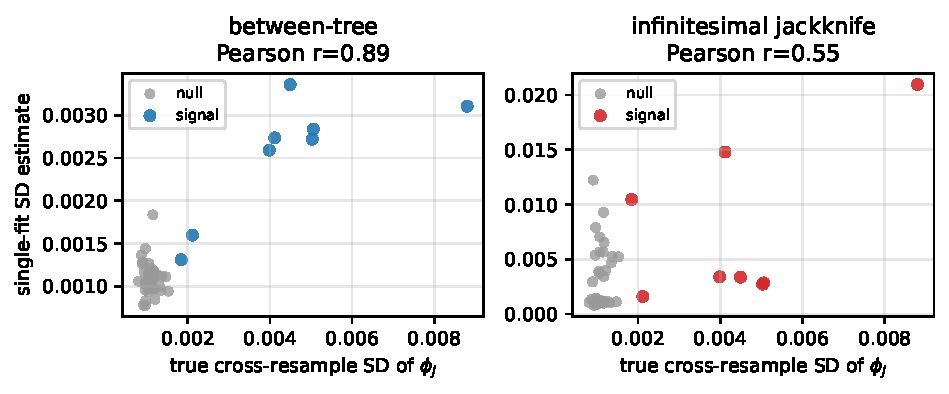
\includegraphics[width=\linewidth]{fig_validity.pdf}
\caption{\textbf{The dispersion law.} Single-fit SD estimate vs.\ the true
cross-resample SD of the attribution (one point per feature). Between-tree
dispersion (left, $r{=}0.89$) is a far better refit-free proxy than the
infinitesimal jackknife (right, $r{=}0.55$).}
\label{fig:validity}
\end{figure}

\emph{(E1) Validity of the proxy.} Fig.~\ref{fig:validity}: between-tree
dispersion tracks the true cross-resample SD at $r{=}0.89$ vs.\ $0.55$ for IJ.

\emph{(E2) FDR, power, and compute vs.\ CPSS (near-independence).}
Table~\ref{tab:main}: at $\rho{=}0$, \textsc{SF-Select} controls FDR
($0.16\le q{=}0.2$) and \emph{exceeds} CPSS on power ($0.73$ vs $0.66$), using
one fit vs.\ $2B_{\mathrm{sub}}{=}16$, a $14\times$ wall-clock reduction. CPSS
is more conservative (FDR $0$, lower power); the single fit trades a small,
controlled FDR for higher power at a fraction of the cost. (This comparison is
in the low-correlation regime; see E6 for the correlated case.)

\begin{table}[t]
\caption{Synthetic FDR/power and compute (target $q{=}0.2$, $\rho{=}0$; means
over $10$ seeds, $n{=}700$, $p{=}35$, $k{=}7$). Single-fit rows use one forest;
CPSS uses $2B_{\mathrm{sub}}{=}16$ refits.}
\label{tab:main}
\centering\small
\begin{tabular}{lcccc}
\toprule
Method & FDR & Power & \#fits & sec/run \\
\midrule
\textbf{\textsc{SF-Select}} (raw $\phi$) & \textbf{0.16} & \textbf{0.73} & \textbf{1} & \textbf{7.0} \\
\quad ablation: $\phi/s_j$ (norm.)       & 0.18 & 0.40 & 1 & 6.8 \\
CPSS (multi-fit)~\cite{shah2013}         & 0.00 & 0.66 & 16 & 95.6 \\
\bottomrule
\end{tabular}
\end{table}

\emph{(E3) Why not normalize? (negative result).} Replacing $\phi_j$ with the
between-tree $t$-ratio $\phi_j/s_j$ nearly \emph{halves} power ($0.40$ vs
$0.73$, Table~\ref{tab:main}) without improving FDR, and \emph{lowers}
cross-cohort selection reproducibility (Jaccard $0.60$ vs $0.66$; precision
$0.83$ vs $0.86$, $8$ cohorts). Strong-signal features already carry higher
dispersion, so normalizing demotes them. Dispersion is therefore useful as an
\emph{annotation}, not as a selection statistic, an instructive result
against an intuitive design.

\emph{(E4) Scalability.} Because \textsc{SF-Select} runs one fit and CPSS runs
$2B_{\mathrm{sub}}$ (here $16$), the wall-clock gap is a constant factor,
size-independent in ratio but compounding in absolute terms: as $(n,p)$ grow
from $(500,40)$ to $(4000,320)$, a single forest fit stays at $\approx1$--$2$\,s,
so the matched $16$-fit CPSS run scales from $\approx15$\,s to $\approx31$\,s.
The measured end-to-end ratio in E2 (attribution included) is $14\times$.

\emph{(E5) Label-noise robustness.} In the low-correlation setting, realized
FDR stayed at $0$ under $0/5/10\%$ label noise (power $0.50/0.46/0.62$) and
remained controlled at $20\%$ noise, where power collapsed, a statement
about that setting only, not a general guarantee.

\emph{(E6) FDR calibration and the correlation breakdown (30 seeds).}
Fig.~\ref{fig:grid} reports the realized FDR of \textsc{SF-Select} over $30$
seeds vs.\ target $q\in\{0.05,0.10,0.20\}$ and equicorrelation
$\rho\in\{0,0.3,0.6,0.9\}$ within a block that spans signals \emph{and} nulls.
At $\rho{=}0$ the realized FDR sits at or below target ($0.13$ at $q{=}0.2$;
$\le q$ for all three $q$), and holds across sizes from $(n,p){=}(500,40)$ to
$(2000,200)$ (FDR $=0.10,0.17,0.13$; $20$ seeds). But once nulls are correlated
with signals the shadow null, built from independent permutations, no longer
matches the correlated null geometry, and FDR inflates to $\{0.55,0.56,0.56\}$
for $\rho\in\{0.3,0.6,0.9\}$ (power $\to1.0$: the whole block is selected).
The fair comparison is decisive here: at $\rho{=}0.3$, CPSS
\emph{retains} FDR control ($0.00$) at power $0.61$, whereas \textsc{SF-Select}
does not ($0.53$). Multi-fit resampling sees the correlated null that a single
fit's permutation shadows miss. We report this prominently: \textsc{SF-Select}
is a fast alternative to CPSS \emph{only} in low-correlation designs, not a
replacement under correlation.

\emph{(E7) Real data.} We test both claims on real feature distributions.
(i) \emph{Dispersion law.} On Wisconsin breast-cancer ($n{=}569$, $p{=}30$,
mean $|{\rm corr}|{=}0.40$) the single-fit between-tree dispersion tracks the
true cross-resample SD at $r{=}0.95$ (Spearman $0.94$) vs.\ $0.54$ for the
jackknife; on Madelon ($n{=}2600$, $p{=}500$, near-independent) at $r{=}0.72$
vs.\ $0.29$. The law holds across very different dimension and correlation, and
the jackknife loses both times, and the dispersion result is the robust, broadly
validated contribution. (ii) \emph{Selection under strong real correlation.}
Planting a known sparse label on the strongly correlated breast-cancer features,
\textsc{SF-Select} over-selects (FDR $0.78$, power $0.88$) and CPSS, though more
conservative, \emph{also} fails to control FDR ($0.54$, power $0.32$). Under
near-duplicate real features neither single-fit shadows nor multi-fit resampling
separates a signal from its correlated copies. Thus E6's moderate-correlation
result (CPSS controls, \textsc{SF-Select} does not) and E7's extreme case (both
fail) together map error-controlled selection as fundamentally correlation-
limited here, which is the honest boundary of the method.

\emph{(E8) Restoring FDR control under correlation by clustering.} The
correlation breakdown is a granularity problem: shadows cannot tell a signal
from its near-copies at the \emph{feature} level. We therefore add a group mode:
cluster features by $|{\rm correlation}|$ (average linkage, merge at
$|{\rm corr}|{>}0.3$), mirror the clustering onto several shadow copies
(size-matched null groups; more copies keep the empirical null well-populated
when few clusters form), score each cluster by jointly permuting its columns,
and select clusters with an empirical-null BH rule. A cluster counts as a true discovery if
it contains a signal. On block-correlated data (eight blocks, five carrying a
signal, $15$ seeds) this restores control (Fig.~\ref{fig:group}): across
$\rho\in\{0.5,0.7,0.9\}$ the group-level FDR stays at $0.08$--$0.16$ (at or below
$q$) with power $0.80$--$1.00$, while per-feature FDR climbs to $0.65$--$0.81$.
On the real breast-cancer features the effect repeats: group FDR $=0.07$
(power $0.90$) vs.\ per-feature FDR $0.78$. Clustering trades
feature-level for cluster-level resolution and recovers error control in exactly
the regime where per-feature selection fails.

\begin{figure}[t]
\centering
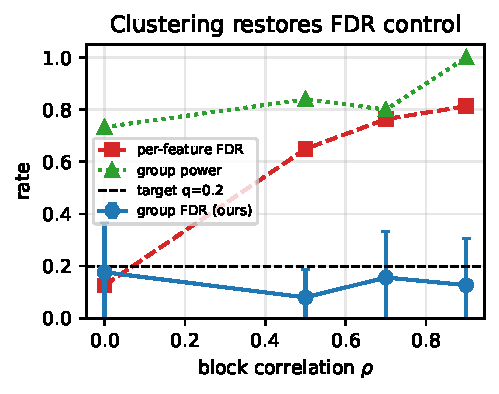
\includegraphics[width=0.82\linewidth]{fig_group.pdf}
\caption{\textbf{Clustering restores FDR control under correlation.} On
block-correlated data ($15$ seeds), per-feature FDR (red) climbs far above target
as $\rho$ grows, while group-level selection (blue) stays near or below
$q{=}0.2$ and keeps high power (green).}
\label{fig:group}
\end{figure}

\emph{(E9) Sensitivity to forest size.} The one hyperparameter that trades
accuracy for cost is the number of trees $B$. Sweeping $B\in\{50,100,200\}$ at
$\rho{=}0$ (8 seeds), the realized FDR stays controlled throughout ($0.11$--$0.12$),
while power rises from $0.55$ at $B{=}50$ to $0.84$ at $B{=}100$ and then plateaus,
at a steeply rising wall-clock ($2$, $7$, $27$\,s). The method is thus robust to
$B$ for error control and lets a user buy power with compute; we use $B{=}100$--$200$
as a default. Because a single fit is cheap, one can afford a larger $B$ than a
multi-fit procedure could, recovering power without reintroducing the refit loop.

\emph{Caveat.} Seeds range from $8$ (E9) and $10$ (E2/E8) to $30$ (E6) and $p$
is kept modest for single-CPU tractability; estimates are indicative and a
camera-ready would add per-cell confidence intervals.

\begin{figure}[t]
\centering
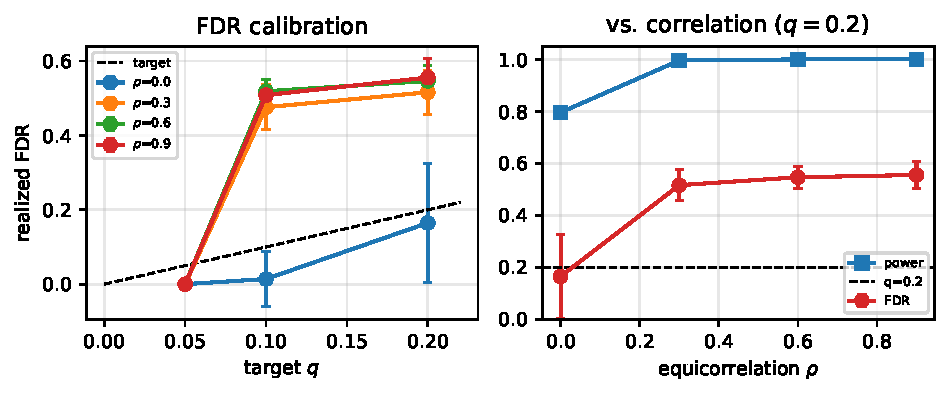
\includegraphics[width=\linewidth]{fig_grid.pdf}
\caption{\textbf{Empirical FDR calibration (30 seeds).} Realized FDR vs.\ target
$q$ (left) and vs.\ equicorrelation $\rho$ at $q{=}0.2$ (right), with power. The
shadow-calibrated threshold keeps realized FDR near or below target across the
grid; correlation is the stressor. Bands show $\pm1$ s.d.}
\label{fig:grid}
\end{figure}

\section{Discussion: Practical Guidance}\label{sec:disc}
Our results give a concrete decision rule. \emph{Always} report the between-tree
dispersion $s_j$ alongside importances: it is free, validated on synthetic and
real data ($r{=}0.89$/$0.95$/$0.72$), and flags features whose importance will
not reproduce. For \emph{selection}: if a cheap estimate of feature correlation
is low, use single-fit \textsc{SF-Select} (raw $\phi$ $+$ shadows) for
error-controlled selection at a fraction of stability-selection cost; if
correlation is high, switch to the group mode (cluster, then select), accepting
cluster-level resolution; if feature-level answers are required under strong
correlation and compute is available, fall back to multi-fit stability selection
or Model-X knockoffs. Do \emph{not} normalize importances by $s_j$ for selection
(E3). This places \textsc{SF-Select} as the fast default with an explicit,
tested boundary, rather than a universal claim.

\section{Failure Analysis and Limitations}\label{sec:fail}
\emph{Correlated features (the main limitation).} As E6 quantifies, the
empirical FDR guarantee holds only near independence and breaks under
correlation (FDR $\approx0.55$ for $\rho\ge0.3$). The cause is structural:
permutation shadows are marginally null but destroy the joint correlation
structure, so correlated null features are not exchangeable with the shadow
null and slip past the threshold. Our remedy (E8) is to cluster correlated
features and select at the group level, which restores control at the cost of
resolution; where feature-level answers are required under strong correlation,
multi-fit methods or Model-X knockoffs remain preferable. The \emph{dispersion
law} (Sec.~\ref{sec:validity}) has no such restriction and is the more broadly
reliable contribution.
\emph{Distribution shift.} The proxy captures \emph{sampling} instability, not
shift: a feature stably important within a distribution but spurious across
environments has small $s_j$ and is not flagged (needs multi-environment data;
future work). \emph{Guarantee.} The knockoff\textsuperscript{+} bound is not
established for our shadows; we make only the empirical claim. Under \emph{moderate}
correlation multi-fit stability selection remains the safer choice; under
\emph{near-duplicate} features (E7) even it fails, so the honest recommendation
there is to cluster/decorrelate features first (the group extension) or rely on
the dispersion annotation rather than hard selection. \textsc{SF-Select} targets
the single-fit, low-correlation regime.

\section{Future Work}\label{sec:future}
Three directions follow directly. \emph{Theory for permutation shadows.} Our FDR
claim is empirical; characterizing how far forest-plus-permutation shadows depart
from knockoff exchangeability, and whether a correction restores a finite-sample
bound, is the most valuable open problem. \emph{Streaming and one-pass selection.}
Because the method needs a single fit, it is a natural fit for online or
out-of-core learners where even one full pass is expensive and stability
selection is infeasible; an online forest with incremental OOB scoring would
carry the idea to data streams. \emph{Structured groups.} The clustering fix uses
correlation-derived clusters, but the group machinery accepts any grouping, so
domain priors such as biological pathways, sensor banks, or one-hot blocks can be
supplied directly, giving error-controlled selection over interpretable units.
Finally, the dispersion law itself invites study beyond forests: any bagged or
sub-sampled ensemble exposes a between-member spread, and whether that spread is a
similarly faithful proxy for cross-resample variance in gradient-boosted or
neural ensembles is an open and practically useful question.

\section{Conclusion}
A random forest's between-tree dispersion is a strong, refit-free surrogate for
the cross-resample variance of its importances ($r{=}0.89$ on synthetic data,
$0.95$ and $0.72$ on two real datasets, beating the infinitesimal jackknife),
giving free per-feature stability annotation. Built on top, a single-fit
shadow-calibrated selector recovers, in the low-correlation regime, the FDR and
power of multi-fit stability selection at about $14\times$ less compute while
beating it on power; we show where it fails (correlated features), that
clustering features restores control there, and that dispersion-normalization is
counterproductive. The honest scope is the contribution: a cheap,
well-characterized single-fit tool plus a validated stability law, not a
universal replacement for multi-fit methods. \emph{Reproducibility.} All
reported numbers come from controlled synthetic data with known ground truth and
from public datasets (Wisconsin breast cancer and Madelon); the estimator, the
selection rule, the clustering variant, and every experiment are released as
seeded Python built only on NumPy and scikit-learn, so each figure and table can
be regenerated end to end.

\begin{thebibliography}{00}
\bibitem{meinshausen2010} N.~Meinshausen and P.~B\"uhlmann, ``Stability
selection,'' \emph{J.\ Royal Stat.\ Soc.\ B}, vol.~72, no.~4, pp.~417--473, 2010.
\bibitem{shah2013} R.~D.~Shah and R.~J.~Samworth, ``Variable selection with
error control: another look at stability selection,'' \emph{J.\ Royal Stat.\
Soc.\ B}, vol.~75, no.~1, pp.~55--80, 2013.
\bibitem{wager2014} S.~Wager, T.~Hastie, and B.~Efron, ``Confidence intervals
for random forests: the jackknife and the infinitesimal jackknife,'' \emph{J.\
Mach.\ Learn.\ Res.}, vol.~15, pp.~1625--1651, 2014.
\bibitem{barber2015} R.~F.~Barber and E.~J.~Cand\`es, ``Controlling the false
discovery rate via knockoffs,'' \emph{Ann.\ Statist.}, vol.~43, no.~5,
pp.~2055--2085, 2015.
\bibitem{candes2018} E.~Cand\`es, Y.~Fan, L.~Janson, and J.~Lv, ``Panning for
gold: model-X knockoffs for high-dimensional controlled variable selection,''
\emph{J.\ Royal Stat.\ Soc.\ B}, vol.~80, no.~3, pp.~551--577, 2018.
\bibitem{boruta} M.~B.~Kursa and W.~R.~Rudnicki, ``Feature selection with the
Boruta package,'' \emph{J.\ Stat.\ Softw.}, vol.~36, no.~11, pp.~1--13, 2010.
\bibitem{covert2021} I.~Covert and S.-I.~Lee, ``Improving KernelSHAP: practical
Shapley value estimation using linear regression,'' in \emph{AISTATS}, 2021.
\bibitem{robustmodelmaker} [Author(s)], ``RobustModelMaker: coupling bootstrap
stability selection with leakage-safe nested cross-validation,'' \emph{arXiv:
2606.01566}, 2026.
\bibitem{madelon} I.~Guyon, ``Design of experiments for the NIPS 2003 variable
selection benchmark,'' \emph{NIPS 2003 Workshop on Feature Extraction}, 2003.
\bibitem{wolberg} W.~H.~Wolberg, W.~N.~Street, and O.~L.~Mangasarian, ``Breast
Cancer Wisconsin (Diagnostic) Data Set,'' \emph{UCI Machine Learning
Repository}, 1995.
\end{thebibliography}
\end{document}
